\documentclass[preprint,12pt,authoryear]{elsarticle}

\usepackage{amsmath,amssymb}
\usepackage{booktabs}
\usepackage{graphicx}
\usepackage{hyperref}
\usepackage{natbib}
\usepackage{float}
\usepackage{multirow}
\usepackage{xcolor}
\usepackage{threeparttable}

\journal{Quantitative Finance}

\begin{document}

\begin{frontmatter}

\title{Temporal Fractal Coupling of Volatility and Trading Volume:\\A Robust Within-Firm Pattern, a Time-Period Stress Signal, and No Firm-Specific Forecast Power in S\&P~500 Stocks, 2015--2026}

\author{Dineshkumar Malempati Hari\corref{cor1}\fnref{orcid}}
\ead{mhdk.dinesh@gmail.com}
\cortext[cor1]{Corresponding author.}
\fntext[orcid]{ORCID: \href{https://orcid.org/0009-0003-1036-9477}{0009-0003-1036-9477}.}

\begin{abstract}
Do the fractal scaling properties of price volatility and trading volume co-evolve, and does their co-movement carry predictive information about future market conditions? I apply detrended fluctuation analysis to 488 current S\&P~500 constituents over 2015--2026, computing rolling Hurst exponents for absolute returns ($H^{(i)}_{|r|,t}$) and log-volume ($H^{(i)}_{v,t}$) in aligned windows, and introduce the Coupling Intensity Index (CII), a rolling Pearson correlation that measures their temporal co-movement. Within-firm temporal coupling is strong and positive: mean $r = 0.531$ across the 488-firm panel, with 92.7\% of firms exhibiting positive coupling and 80.4\% above $r = 0.3$. The pattern holds across all eleven GICS sectors. Coupling heterogeneity rises sharply in high-VIX regimes (Mann-Whitney high vs.\ low $p = 0.0019$, with the upper-quartile distribution exhibiting both higher medians and substantially greater dispersion), but mean coupling does not uniformly intensify with stress. The predictive question is more nuanced. Under inference robust to two-way clustering by firm and time \citep{cameron2011robust}, Bell--McCaffrey CR2 with Satterthwaite degrees of freedom \citep{imbens2016robust}, and the wild cluster restricted bootstrap \citep{mackinnon2017wild}, CII has no firm-specific incremental predictive content for forward standard dollar-volume Amihud \citep{amihud2002illiquidity} illiquidity, the Corwin--Schultz spread \citep{corwin2012simple}, the Roll spread \citep{roll1984spread}, realised volatility, or six other liquidity proxies. Inference methods that condition on the time dimension instead (time-clustered standard errors, Driscoll--Kraay HAC) detect a significant cross-firm time-period co-movement that the firm-conditional methods do not. The natural reading is that CII inherits a market-wide stress signal that moves with forward liquidity proxies in aggregate but adds no firm-specific predictive content beyond what the standard liquidity-and-volatility toolkit already captures; every focal-only signal in the battery is fully absorbed by nine standard benchmarks in the combined horse-race specification. An apparently strong predictive result against a non-standard share-volume illiquidity proxy dissipates once both proper Amihud convention and dependence-robust inference are imposed; I document and dissect this as a price-level confound. The contribution is therefore a robust within-firm fractal coupling phenomenon, a sharp absorption pattern that pinpoints the dimension of dependence carrying CII's apparent signal, and two methodological cautions for the wider econophysics-meets-finance literature: distinguish share-volume from dollar-volume liquidity proxies, and report whichever inference dimension matches the unit of analysis the paper actually claims.
\end{abstract}

\begin{keyword}
Hurst exponent \sep Detrended fluctuation analysis \sep Price-volume relationship \sep Long memory \sep Coupling Intensity Index \sep Amihud illiquidity \sep Cluster-robust inference \sep Wild cluster bootstrap \sep Methodological caveat
\end{keyword}

\end{frontmatter}

% ============================================================
\section{Introduction}
\label{sec:intro}
% ============================================================

Financial price volatility and trading volume each exhibit long-range dependence.\footnote{This paper builds on an earlier MSc project \citep{hari2013fractal} in which I examined whether Hurst-based fractal characteristics of stock-price series were associated with average trading volume in the cross section. That earlier work found a weak but statistically significant static relationship. The present study extends that line of inquiry by shifting from static association to temporal co-evolution, asking whether the persistence structures of volatility and volume move together through time and whether that coupling predicts future market illiquidity.} Absolute returns display Hurst exponents of approximately 0.7--0.8 \citep{ding1993long, bollerslev1999equity}, while volume persists even more strongly at $H \approx 0.7$--0.9 \citep{lobato2000long}. Whether these two fractal regimes are \emph{coupled} (whether they co-evolve over time, and whether that co-evolution carries information a financial economist would care about) has not been systematically investigated.

This paper addresses both questions. I distinguish between \emph{static} coupling (the cross-sectional correlation of Hurst exponents across firms) and \emph{temporal} coupling (the within-firm co-movement of rolling Hurst exponents over time), and I construct a Coupling Intensity Index (CII) that measures the strength of temporal coupling as a time-varying quantity. I then test four hypotheses:

\begin{itemize}
\item[\textbf{H1}] \emph{Static coupling:} Firms with more persistent volume also have more persistent volatility in the cross-section.
\item[\textbf{H2}] \emph{Temporal coupling:} Rolling Hurst exponents for $|r_t|$ and $\log V_t$ co-move positively within firms over time.
\item[\textbf{H3}] \emph{Regime dependence:} Temporal coupling intensifies during high-uncertainty regimes (elevated VIX).
\item[\textbf{H4}] \emph{Predictive content:} CII has incremental predictive content for standard forward liquidity and volatility measures.
\end{itemize}

The results are as follows. H1 is rejected: the cross-sectional correlation between full-sample $H_{|r|}$ and $H_v$ is null. H2 is strongly supported at the full S\&P~500 scale: mean within-firm temporal coupling is $r = 0.531$, with 92.7\% of the 488 panel firms exhibiting positive coupling and 80.4\% above $r = 0.3$; the pattern is universal across all eleven GICS sectors. H3 is confirmed in a sharper form than its original 50-firm version: a Mann-Whitney test for the high-VIX vs.\ low-VIX coupling distribution rejects the null at $p = 0.0019$, but the rejection is driven by distributional shape rather than mean shift. The high-VIX regime exhibits a higher median of within-firm coupling and substantially greater cross-firm dispersion; mean coupling does not uniformly intensify with stress.

H4, by contrast, is rejected for firm-specific predictive content but exhibits a structural inference disagreement that is itself informative. Under inference methods that condition on the firm dimension (firm-clustered, two-way clustered with the Cameron--Gelbach--Miller eigenvalue PSD adjustment, Bell--McCaffrey CR2, and the wild cluster restricted bootstrap), CII has no incremental predictive content for forward Amihud illiquidity computed in the standard dollar-volume convention of \citet{amihud2002illiquidity}, nor for realised volatility, the Corwin--Schultz spread, the Roll spread, the volatility of realised volatility, the maximum drawdown, abnormal turnover, log Amihud, or $\Delta$Amihud. Inference methods that condition on the time dimension instead (time-clustered standard errors, Driscoll--Kraay HAC) detect a statistically significant cross-firm time-period co-movement between CII and several forward liquidity proxies. The horse race against nine standard liquidity benchmarks is decisive: every focal-only signal in the battery is fully absorbed in the combined specification (the strongest case is the forward Corwin--Schultz spread, where focal two-way $t = +3.64$ collapses to combined $t = +0.07$). The reading is that CII inherits a market-wide stress co-movement that moves with several forward liquidity proxies in aggregate but adds no firm-specific predictive content beyond what the standard toolkit already captures.

A specification that uses share volume rather than dollar volume in the Amihud denominator does produce a statistically significant CII coefficient at $G = 50$ and survives the wild cluster restricted bootstrap. That signal disappears once dollar volume replaces share volume in the denominator, as standard practice requires. Section~\ref{sec:h4_diagnosis} dissects the divergence as a price-level confound: the share-volume Amihud co-moves with within-firm price-level drift, and CII correlates with that drift component rather than with price impact per dollar traded. The fix is in the dependent-variable definition rather than in the standard errors, and modern cluster-robust inference (including the wild cluster bootstrap) does not detect it.

This combination of results is sharper than the broad predictive thesis the paper originally set out to test. Prior work on price-volume fractal relationships \citep{podobnik2009cross} and common long-memory components \citep{bollerslev1999equity} has established that volatility and volume share structural features. The present paper shows that the within-firm coupling of those structural features (a) exists in a strong and quantitatively measurable form across the full S\&P~500, (b) is regime-dependent in a heterogeneity-amplifying rather than mean-amplifying sense, (c) carries no firm-specific predictive content for standard market-quality outcomes once the firm dimension of dependence is properly modelled, and (d) co-moves with cross-firm time-period stress dynamics in ways that several inference methods detect but that horse-race conditioning fully absorbs. The empirical claim is narrower than the original H4 but is structurally informative: the inference-method disagreement pinpoints exactly which dimension of dependence carries the apparent signal and which does not. The paper also delivers two transferable cautionary lessons: distinguish share-volume from dollar-volume illiquidity proxies, and report inference at the dimension that matches the unit of analysis the paper actually claims, since the choice can determine whether one finds a signal or a null at the same data.

The conceptual distinction that organises the paper is between first-order and second-order fractal properties. Detrended cross-correlation analysis (DCCA; \citealp{podobnik2008detrended}) measures whether price and volume fluctuations are correlated at different scales, a first-order property. The rolling Hurst approach measures whether the \emph{scaling exponents themselves} (which summarise how memory decays) evolve in tandem. This is a second-order property: a statement about the dynamics of complexity rather than the dynamics of levels.

% ============================================================
\section{Literature}
\label{sec:literature}
% ============================================================

\subsection{Long Memory in Returns and Volatility}

\citet{mandelbrot1963variation} first demonstrated that financial prices exhibit non-Gaussian, scale-invariant properties. The Hurst exponent $H$, originally developed for hydrological applications \citep{hurst1951long} and formalised through fractional Brownian motion \citep{mandelbrot1968fractional}, provides the standard measure of long-range dependence. \citet{cont2001empirical} identified the slow decay of autocorrelation in absolute returns as among the most robust stylised facts in finance. \citet{ding1993long} showed that this long memory is strongest for $|r_t|^d$ at $d \approx 1$, persisting over hundreds of lags. \citet{lo1991long} cautioned that naive R/S analysis can overstate long memory when short-range dependence is present, motivating the use of detrended fluctuation analysis \citep{peng1994mosaic}. Finite-sample properties and heavy-tail biases have been characterised by \citet{weron2002estimating} and \citet{barunik2010hurst}. The HAR-RV model of \citet{corsi2009simple} provides an influential parsimonious framework for realised volatility forecasting, exploiting the heterogeneous autoregressive structure of realised measures.

\subsection{Long Memory in Trading Volume}

\citet{lobato2000long} provided rigorous evidence for fractional integration in volume, estimating $H \approx 0.7$--$0.9$ across NYSE equities. This finding is even more robust than the volatility long-memory result and has been replicated across markets and frequencies. \citet{plerou2003two} documented power-law correlations between price changes and volume, while \citet{ray2000long} confirmed long-range dependence in daily stock volatilities. \citet{chordia2001trading} showed that trading activity predicts expected stock returns through its relationship to liquidity provision.

\subsection{Liquidity, Volume, and Market Microstructure}

The Amihud illiquidity ratio \citep{amihud2002illiquidity} has become a standard measure of price impact per unit of trading volume, capturing the adverse-selection component of illiquidity. \citet{kyle1985continuous} provided the theoretical foundation for relating information asymmetry to market depth. \citet{brunnermeier2009market} formalised the feedback loop between volatility and liquidity: when volatility rises, margins tighten, forcing deleveraging that further reduces liquidity. This volatility-liquidity spiral provides a theoretical channel through which fractal coupling between volatility persistence and volume persistence could predict liquidity deterioration.

\subsection{Joint Dynamics: The MDH and Beyond}

The Mixture of Distributions Hypothesis \citep{clark1973subordinated, tauchen1983price, epps1976stochastic} posits a latent information arrival process that simultaneously governs volatility and volume. \citet{andersen1996return} recast the MDH within a stochastic volatility framework, showing time-varying information flow generates the observed co-clustering. \citet{bollerslev1999equity} identified a common long-memory component shared by volatility and volume using ARFIMA methods. \citet{podobnik2009cross} applied DCCA to measure scale-dependent cross-correlations between price changes and volume changes. \citet{karpoff1987relation} and \citet{gallant1992stock} established the broader empirical price-volume relationship. \citet{kristoufek2015power} reviewed the methodological challenges and open problems in measuring power-law cross-correlations, including bias and finite-sample issues that motivate the rolling-window approach adopted here.

Several studies have computed time-varying Hurst exponents for individual series: \citet{cajueiro2004hurst} for emerging-market efficiency, \citet{alvarez2008time} for U.S.\ indices, \citet{grech2004crash} for crash prediction. None, however, examines whether Hurst exponents computed from \emph{two distinct series} co-move through time, nor whether such co-movement predicts economically relevant outcomes. This is the gap the present study addresses.

% ============================================================
\section{Methodology}
\label{sec:methods}
% ============================================================

\subsection{Detrended Fluctuation Analysis}

For a time series $\{x_t\}_{t=1}^{N}$, the cumulative deviation profile is $Y(k) = \sum_{t=1}^{k}(x_t - \bar{x})$. The profile is divided into non-overlapping windows of length $s$, each detrended by a fitted polynomial of order $m$ (here $m = 1$, i.e., DFA-1). The fluctuation function is:
\begin{equation}
F(s) = \left[ \frac{1}{N_s} \sum_{\nu=1}^{N_s} \frac{1}{s} \sum_{k=1}^{s} \left( Y((\nu-1)s + k) - \tilde{Y}_\nu(k) \right)^2 \right]^{1/2}.
\end{equation}
For a long-range correlated process, $F(s) \sim s^H$. The Hurst exponent $H$ is estimated as the ordinary least squares slope of $\log F(s)$ versus $\log s$. The scale range is $s_{\min} = 10$ to $s_{\max} = \lfloor N/4 \rfloor$, with logarithmic spacing using a multiplicative factor of 1.2 (i.e., scales $s_k = \lfloor s_{\min} \times 1.2^k \rfloor$ for $k = 0, 1, 2, \ldots$ up to $s_{\max}$). Fit quality is assessed via $R^2$ of the log-log regression.

\subsection{Series Construction}

For each equity $i$, three series are constructed from daily close prices $P_t^{(i)}$ and volumes $V_t^{(i)}$:
\begin{align}
r_t^{(i)} &= \log P_t^{(i)} - \log P_{t-1}^{(i)}, \\
|r_t^{(i)}| &= |\log P_t^{(i)} - \log P_{t-1}^{(i)}|, \\
v_t^{(i)} &= \log(V_t^{(i)} + 1).
\end{align}
Stationarity is verified via the ADF and KPSS tests. All log-return series are confirmed stationary.

\subsection{Rolling Hurst Exponents}
\label{sec:rolling_hurst}

The rolling Hurst exponent at time $t$ for window length $W$ and step size $\Delta$ is defined as:
\begin{equation}
H^{(i)}_{|r|,t} = \mathrm{DFA}\!\left(\{|r_\tau^{(i)}|\}_{\tau=t-W+1}^{t}\right), \quad H^{(i)}_{v,t} = \mathrm{DFA}\!\left(\{v_\tau^{(i)}\}_{\tau=t-W+1}^{t}\right),
\end{equation}
where $H^{(i)}_{|r|,t}$ denotes the Hurst exponent of absolute returns (the volatility proxy) and $H^{(i)}_{v,t}$ denotes the Hurst exponent of log-volume for firm $i$ at rolling index $t$. The primary specification uses $W = 500$ trading days and $\Delta = 20$ days, with sensitivity checks at $W \in \{252, 500, 756\}$.

\subsection{Coupling Metrics}

\textbf{Static coupling} is the cross-sectional Pearson correlation of full-sample $H^{(i)}_{|r|}$ and $H^{(i)}_{v}$ computed across all $i = 1, \ldots, 50$ firms.

\textbf{Temporal coupling} for firm $i$ is the Pearson correlation computed over the full set of rolling indices:
\begin{equation}
\rho^{(i)} = \mathrm{Corr}\!\left(H^{(i)}_{|r|,t},\, H^{(i)}_{v,t}\right), \quad t \in \mathcal{T}^{(i)},
\end{equation}
where $\mathcal{T}^{(i)}$ is the discrete set of rolling-window evaluation dates for firm $i$.

\textbf{Coupling Intensity Index (CII).} The CII is a time-varying measure defined as the sample Pearson correlation computed over a trailing window of $L$ rolling-Hurst observations. Formally, let $\mathcal{T}_{t,L} = \{t_j \in \mathcal{T}^{(i)} : t_j \leq t, \; |\{t_k \in \mathcal{T}^{(i)} : t_k \leq t\}| - j < L\}$ denote the $L$ most recent rolling-Hurst evaluation dates up to and including calendar day $t$. Then:
\begin{equation}
\mathrm{CII}^{(i)}_t = \frac{\sum_{j \in \mathcal{T}_{t,L}} \bigl(H^{(i)}_{|r|,j} - \bar{H}^{(i)}_{|r|}\bigr)\bigl(H^{(i)}_{v,j} - \bar{H}^{(i)}_{v}\bigr)}{\sqrt{\sum_{j \in \mathcal{T}_{t,L}} \bigl(H^{(i)}_{|r|,j} - \bar{H}^{(i)}_{|r|}\bigr)^2 \; \sum_{j \in \mathcal{T}_{t,L}} \bigl(H^{(i)}_{v,j} - \bar{H}^{(i)}_{v}\bigr)^2}},
\label{eq:cii}
\end{equation}
where $\bar{H}^{(i)}_{|r|}$ and $\bar{H}^{(i)}_{v}$ are the sample means over $\mathcal{T}_{t,L}$. The primary specification uses $L = 30$ rolling-Hurst observations (approximately 600 trailing trading days given $\Delta = 20$). Sensitivity to $L \in \{20, 30, 40\}$ is reported below.

\textbf{Timing convention.} $\mathrm{CII}^{(i)}_t$ is computable at the close of trading day $t$ and uses only data through day $t$. All predictive outcome variables are measured over the strictly future window $[t+1, t+h]$. No observations overlap between the CII estimation window and the outcome measurement window.

\subsection{Predictive Regression}
\label{sec:pred_reg}

To test H4, I estimate panel regressions with firm fixed effects:
\begin{equation}
Y^{(i)}_{t+h} = \alpha_i + \beta_1 \, \mathrm{CII}^{(i)}_t + \beta_2 \, H^{(i)}_{|r|,t} + \beta_3 \, H^{(i)}_{v,t} + \varepsilon^{(i)}_t,
\label{eq:panel}
\end{equation}
where $Y^{(i)}_{t+h}$ is a forward-looking outcome measured over $[t+1, t+h]$:
\begin{itemize}
\item \emph{Amihud illiquidity} \citep{amihud2002illiquidity}, dollar-volume convention scaled by $10^{6}$: $\mathrm{ILLIQ}^{(i)}_{t+h} = \frac{10^{6}}{h}\sum_{\tau=t+1}^{t+h} \frac{|r^{(i)}_\tau|}{V^{(i)}_\tau \cdot P^{(i)}_\tau}$
\item \emph{Realised volatility}: $\mathrm{RV}^{(i)}_{t+h} = \sqrt{\sum_{\tau=t+1}^{t+h} (r^{(i)}_\tau)^2}$
\item \emph{Abnormal turnover}: forward share volume normalised by trailing 60-day mean
\item \emph{Maximum drawdown}: largest peak-to-trough decline in $[t+1, t+h]$
\end{itemize}
The dollar-volume denominator $V^{(i)}_\tau \cdot P^{(i)}_\tau$ is the standard Amihud convention. An earlier version of this study used share volume in the denominator and produced a statistically significant CII coefficient that does not survive the standard convention; Section~\ref{sec:h4_diagnosis} treats this as a substantive finding in its own right.

Amihud illiquidity is the \emph{primary} H4 outcome of the paper. The remaining three (realised volatility, abnormal turnover, maximum drawdown) and the further proxies introduced in Section~\ref{sec:h4} (Corwin--Schultz spread, Roll spread, vol-of-vol, $\log$ Amihud, and forward $\Delta$Amihud) are reported as \emph{exploratory secondary outcomes}. Because all ten outcomes return statistically null estimates for the focal $\beta_1$ coefficient, family-wise multiple-testing corrections would only widen the reported $p$-values further from significance and are omitted as redundant. Horizons are $h \in \{5, 21\}$ trading days (one week, one month).

Because panel observations are likely correlated both within firms (persistence) and within time periods (common shocks), I report five baseline standard-error specifications: heteroskedasticity-consistent (HC1), clustered by firm, clustered by time, two-way clustered by firm and time following \citet{cameron2011robust}, and Newey-West with automatic bandwidth selection \citep{newey1987simple}. The two-way clustered specification accounts for both within-firm persistence and cross-sectional correlation from common shocks. For the combined horse-race specification (Section~\ref{sec:horse_race}) I additionally report two small-sample corrections recommended in modern cluster-robust practice: the Bell--McCaffrey CR2 standard error with Satterthwaite effective degrees of freedom \citep{imbens2016robust}, and the wild cluster restricted bootstrap with Rademacher weights following \citet{cameron2008bootstrap} and \citet{mackinnon2017wild}. These provide stricter inference than the asymptotic CRVE at $G = 50$ firms; details are in Section~\ref{sec:horse_race} and Table~\ref{tab:horserace_smallsample}. The coefficient of interest is $\beta_1$: does CII predict future outcomes \emph{beyond} what the individual Hurst levels already capture?

\subsection{Regime Conditioning}

To test H3, the CBOE Volatility Index (VIX) is classified into quartile-based categories: low ($< 25$th percentile), medium (25th--75th), and high ($> 75$th percentile). Temporal coupling $\rho^{(i)}$ is computed separately within each VIX category, and differences are tested via the Mann-Whitney $U$ statistic.

\subsection{Robustness}

Eleven checks are conducted: window sensitivity ($W \in \{252, 500, 756\}$), non-overlapping windows, first-differenced Hurst series, shuffled surrogates, squared returns as alternative volatility proxy, subperiod analysis, sector decomposition, market factor control (partial correlation after removing SPY Hurst dynamics), DFA polynomial order (linear vs.\ quadratic), alternative estimators (R/S, MFDFA at $q = 2$), and Granger causality between the two Hurst series. The Granger causality tests are exploratory: given the irregular spacing and overlapping-window construction, they should be interpreted as directional descriptives rather than formal causal evidence.

% ============================================================
\section{Data}
\label{sec:data}
% ============================================================

The sample comprises the 488 S\&P~500 constituents (out of 503 attempted) for which Yahoo Finance returned at least 600 daily observations and the log-return series passed both ADF ($p < 0.01$) and KPSS ($p > 0.10$) stationarity tests over January 2, 2015 through April 1, 2026 ($\approx 2{,}800$ observations per equity). The universe spans all eleven GICS sectors. Constituency is current as of April 2026; the resulting sample inherits a survivorship-bias profile typical of contemporary S\&P~500 universes and shared with most prior work using the same construction. VIX data are obtained from the CBOE via Yahoo Finance.

An earlier version of this study used a smaller 50-firm sample of large-cap S\&P~500 names (v1.0--v1.2). The 488-firm panel reported here was added to test whether the small-sample inference observed at $G = 50$ was a power constraint or a robust feature of the data; that question is addressed in Section~\ref{sec:horse_race}.

% ============================================================
\section{Results}
\label{sec:results}
% ============================================================

\subsection{Baseline Hurst Estimates}

Figure~\ref{fig:distributions} displays the distribution of full-sample estimates from the v1.0--v1.2 50-firm sample, which is mechanically the same DFA construction as the 488-firm panel. $H(\text{returns})$ averages 0.461, confirming approximate market efficiency. $H^{(i)}_{|r|}$ averages 0.795, and $H^{(i)}_{v}$ averages 0.881, replicating the canonical long-memory findings. Log-log fit quality is excellent (mean $R^2 = 0.994$; Figure~\ref{fig:loglog}). Bootstrap confidence intervals confirm $H \neq 0.5$ at $p < 0.001$ on both volatility and volume.

\subsection{H1: Static Coupling (Rejected)}

The cross-sectional Pearson correlation between $H^{(i)}_{|r|}$ and $H^{(i)}_{v}$ is $r = -0.02$ ($p = 0.88$; Figure~\ref{fig:cross_sectional}). Spearman $\rho = 0.03$ ($p = 0.85$). \textbf{H1 is rejected.} The cross-section does not reveal a meaningful relationship in this sample: a stock's volatility persistence tells you nothing about its volume persistence.

\subsection{H2: Temporal Coupling (Confirmed)}

Across the 488-firm S\&P~500 panel, the mean within-firm temporal Pearson correlation is $\bar{\rho} = 0.531$, with median 0.615, 92.7\% of firms exhibiting positive coupling, 80.4\% above $r = 0.3$, and 64.5\% above $r = 0.5$. The minimum is $r = -0.570$ and the maximum is $r = 0.974$. \textbf{H2 is strongly confirmed.}

Sector decomposition shows the phenomenon is universal across the eleven GICS sectors: Energy leads at mean $r = 0.660$ (95.5\% positive), followed by Consumer Discretionary (0.626, 95.8\%), Financials (0.610, 94.7\%), Health Care (0.543, 94.6\%), Consumer Staples (0.541, 97.1\%), Industrials (0.530, 92.2\%), Communication Services (0.476, 87.0\%), Information Technology (0.471, 91.5\%), Real Estate (0.461, 87.1\%), Materials (0.425, 92.3\%), and Utilities (0.412, 87.1\%). Every sector has at least 87\% of firms with positive coupling.

The original 50-firm sample (large-cap focus, v1.0--v1.2) reported a slightly stronger mean ($\bar\rho = 0.665$, 49 of 50 firms positive). The G = 488 mean is closer to the lower end of the cross-sector distribution because the broader universe includes mid-cap and recently-added firms with lower coupling magnitudes. The phenomenon is strongest in large-cap names but holds across the full S\&P~500 constituency.

Figure~\ref{fig:rolling} illustrates the co-movement for AAPL ($r = 0.759$), JPM ($r = 0.901$), and META ($r = -0.421$, the most extreme negative case in the original 50-firm sample, coinciding with the firm's 2022--23 corporate restructuring). The lead-lag profile (Figure~\ref{fig:leadlag}) peaks at lag zero and decays symmetrically, consistent with a shared contemporaneous driver.

Exploratory Granger causality tests on the 50-firm subsample revealed a directional asymmetry: volume persistence Granger-causes volatility persistence in 26\% of tickers versus 8\% in the reverse direction. While this three-fold asymmetry is suggestive of information manifesting first in trading activity \citep{gallant1992stock, kyle1985continuous}, the overlapping-window construction limits the strength of causal claims from these tests; the result is reported as exploratory and was not re-run on the full 488-firm panel.

\subsection{H3: Regime Dependence (Confirmed in Distribution Shape)}

Temporal coupling conditioned on VIX quartile-based categories at $G = 488$:

\begin{table}[H]
\centering
\begin{tabular}{lcccc}
\toprule
VIX Category & Mean $\rho$ & Median $\rho$ & Std & $n$ firms \\
\midrule
Low ($< 25$th pctile) & 0.567 & 0.666 & 0.344 & 495 \\
Medium (25th--75th) & 0.497 & 0.566 & 0.299 & 495 \\
High ($> 75$th pctile) & 0.563 & 0.738 & 0.450 & 495 \\
\bottomrule
\end{tabular}
\caption{Temporal coupling by VIX regime, $G = 488$. Mann-Whitney test (high $>$ low) on the cross-firm distributions: $U = 135{,}542$, $p = 0.0019$.}
\label{tab:vix_regime}
\end{table}

\noindent \textbf{H3 is confirmed.} Coupling is significantly higher during high-VIX periods. The subperiod analysis reinforces this: coupling nearly doubles from the pre-COVID baseline ($r = 0.41$) to the crisis period ($r = 0.77$; Figure~\ref{fig:subperiod}), then attenuates post-crisis ($r = 0.30$).

\subsection{H4: Predictive Content (Firm-Specific Null, Time-Period Co-Movement)}
\label{sec:h4}

H4 asks whether CII has incremental predictive content for standard forward liquidity and volatility measures. The answer, after running ten target specifications across six baseline standard-error methods plus two small-sample corrections at $G = 488$, is structured: under inference methods that condition on the firm dimension (firm-clustered, two-way clustered, Bell--McCaffrey CR2 with Satterthwaite df, the wild cluster restricted bootstrap), the CII coefficient is statistically null for every target in every specification. Under inference methods that condition on the time dimension instead (time-clustered standard errors, Driscoll--Kraay HAC), several focal-only signals reach the 5\% threshold for the primary outcome and for five of the eight secondary outcomes. The horse race against nine standard liquidity benchmarks is decisive: every focal-only signal in the battery is fully absorbed in the combined specification, regardless of which SE method is used.

The natural reading is that CII inherits a market-wide stress co-movement that affects multiple forward liquidity proxies in aggregate, but adds no firm-specific predictive content beyond what the standard liquidity-and-volatility toolkit already captures. The inference disagreement pinpoints exactly which dimension of dependence carries the apparent signal: the cross-firm time-period dimension, not the firm-specific dimension. Section~\ref{sec:h4_diagnosis} below additionally explains why an earlier version of this study using share-volume Amihud reported a robust positive result: it was driven by a price-level component of the non-standard denominator, not by predictive content for price impact per dollar traded. Section~\ref{sec:cluster_heterogeneity} addresses the third methodological observation of this paper: the Bell--McCaffrey CR2 Satterthwaite effective degrees of freedom collapsed to 1.0 at $G = 488$, which carries practical implications for cluster-robust inference in panels with leverage-heterogeneous firms.

\subsubsection{Primary Specification: Forward Amihud Illiquidity}

Table~\ref{tab:predictive} reports panel regression results for Equation~\eqref{eq:panel} at the one-month horizon ($h = 21$) on the 488-firm panel. The dependent variable is the standard Amihud illiquidity defined in Section~\ref{sec:pred_reg} with dollar volume in the denominator.

\begin{table}[H]
\centering
\begin{threeparttable}
\caption{Inference for CII $\to$ standard (dollar-volume) Amihud illiquidity, $G = 488$, focal specification with Hurst controls ($h = 21$ trading days).}
\label{tab:predictive}
\begin{tabular}{lrrr}
\toprule
SE Method & $t$-statistic & $p$-value & df \\
\midrule
HC1 (White) & $-2.56$ & 0.011 & 41{,}569 \\
Firm-clustered & $-0.92$ & 0.357 & 487 \\
Time-clustered & $\mathbf{-2.61}$ & $\mathbf{0.011}$ & 83 \\
Two-way clustered & $-0.93$ & 0.356 & 83 \\
Newey--West & $-1.48$ & 0.138 & 41{,}569 \\
Driscoll--Kraay & $\mathbf{-2.25}$ & $\mathbf{0.025}$ & 872 \\
Bell--McCaffrey CR2 & $-0.91$ & 0.527 & df$_\mathrm{satt}$ = 1.02 \\
WCR bootstrap & --- & 0.720 & $n_\mathrm{boot}$ = 999 \\
\bottomrule
\end{tabular}
\begin{tablenotes}
\small
\item Panel regressions with firm fixed effects, $N = 41{,}572$ observations across 488 equities and 875 calendar months. Regressors: $\mathrm{CII}^{(i)}_{t}$, $H^{(i)}_{|r|,t}$, $H^{(i)}_{v,t}$. Two-way clustering follows \citet{cameron2011robust} with the eigenvalue PSD adjustment of CGM (2011) \S2.3 applied when needed. Driscoll--Kraay uses Bartlett bandwidth $\geq 21$ \citep{driscoll1998consistent}. CR2 follows \citet{imbens2016robust} at the firm dimension; WCR follows \citet{cameron2008bootstrap} and \citet{mackinnon2017wild} with Rademacher weights and the restricted null. Bold rows mark methods that detect a significant CII coefficient at the 5\% level.
\end{tablenotes}
\end{threeparttable}
\end{table}

The CII coefficient is $\hat{\beta}_{\mathrm{CII}} = -2.6 \times 10^{-3}$. The disagreement between firm-conditional methods (firm-clustered, two-way, CR2, WCR) and time-conditional methods (time-clustered, Driscoll--Kraay) is structural rather than ad hoc. Methods that allow within-firm correlation but not within-time correlation see a null because the apparent signal lives in the cross-firm time-period dimension. Methods that allow within-time correlation see a $t$ near $-2.5$ because that cross-firm dimension is real. The two-way clustered specification, which allows both, attributes the shared variance to the larger of the two cluster sets and ends up null. The natural interpretation: the CII coefficient on forward Amihud reflects co-movement of CII and Amihud at the cross-firm time-period level (a market-wide stress dynamic), not within-firm one-month-ahead forecasting power. Whether one calls this ``predictive content'' is a matter of definition; under the standard asset-pricing definition, where the unit of forecast is firm-month, the result is null.

\subsubsection{Battery of Standard Liquidity and Volatility Outcomes}

Table~\ref{tab:battery} extends the test to nine target variables (the primary plus eight secondary outcomes), each in both focal and combined specifications.

\begin{table}[H]
\centering
\begin{threeparttable}
\caption{Predictive battery, $G = 488$: CII coefficient and inference for nine target specifications, focal and combined-with-9-benchmarks regressions, $h = 21$.}
\label{tab:battery}
\begin{tabular}{lrrrrr}
\toprule
Target & $\hat{\beta}^{\mathrm{focal}}_{\mathrm{CII}}$ & $t^{\mathrm{focal}}_{\mathrm{2way}}$ & $t^{\mathrm{focal}}_{\mathrm{DK}}$ & $t^{\mathrm{combined}}_{\mathrm{2way}}$ & $t^{\mathrm{combined}}_{\mathrm{DK}}$ \\
\midrule
\multicolumn{6}{l}{\emph{Standard Amihud and transformations}} \\
\quad Amihud illiquidity (PRIMARY) & $-2.6\!\times\!10^{-3}$ & $-0.93$ & $\mathbf{-2.25^{*}}$ & $-0.77$ & $-1.75$ \\
\quad $\log$ Amihud & $+0.071$ & $\mathbf{+2.19^{*}}$ & $+1.92$ & $+0.21$ & $+0.21$ \\
\quad $\Delta$Amihud & $-4.4\!\times\!10^{-4}$ & $-1.61$ & $-0.56$ & $-0.96$ & $-0.97$ \\
\midrule
\multicolumn{6}{l}{\emph{Spread-based liquidity proxies}} \\
\quad Forward Corwin--Schultz spread & $+5.1\!\times\!10^{-4}$ & $\mathbf{+3.64^{**}}$ & $\mathbf{+3.45^{**}}$ & $+0.07$ & $+0.10$ \\
\quad Forward Roll spread & $+1.2\!\times\!10^{-3}$ & $\mathbf{+2.07^{*}}$ & $\mathbf{+1.99^{*}}$ & $+0.62$ & $+0.76$ \\
\midrule
\multicolumn{6}{l}{\emph{Other forward outcomes}} \\
\quad Forward vol-of-vol & $+4.7\!\times\!10^{-3}$ & $+1.40$ & $+1.13$ & $-1.11$ & $-1.87$ \\
\quad Realised volatility & $+6.7\!\times\!10^{-3}$ & $\mathbf{+2.49^{*}}$ & $\mathbf{+2.33^{*}}$ & $+0.08$ & $+0.10$ \\
\quad Maximum drawdown & $-6.3\!\times\!10^{-3}$ & $-1.74$ & $-1.83$ & $-0.81$ & $-0.92$ \\
\quad Abnormal turnover & $+0.254$ & $+1.03$ & $+1.01$ & $+1.08$ & $+1.04$ \\
\bottomrule
\end{tabular}
\begin{tablenotes}
\small
\item Panel regressions with firm fixed effects. Focal regressors: $\mathrm{CII}^{(i)}_t$, $H^{(i)}_{|r|,t}$, $H^{(i)}_{v,t}$. Combined adds the nine standard benchmarks listed in Table~\ref{tab:horserace}. Two-way clustered SEs (Cameron--Gelbach--Miller 2011) and Driscoll--Kraay SEs (Bartlett bandwidth $\geq 21$) are reported. Bold cells mark $p < 0.05$. ${}^{*}\,p < 0.05$; ${}^{**}\,p < 0.01$. The pattern is uniform: focal-only coefficients that reach significance for the primary outcome and for five of eight secondaries are absorbed to null in the combined specification across both SE methods. The forward Corwin--Schultz spread illustrates the absorption most cleanly ($t = +3.64 \to +0.07$, four-orders-of-magnitude drop in the coefficient).
\end{tablenotes}
\end{threeparttable}
\end{table}

Reading the table: at $G = 488$, several focal-only specifications cross the 5\% threshold under two-way clustering or Driscoll--Kraay HAC. Every single focal-significant coefficient becomes statistically null in the combined specification. The implication is identical for all nine targets: CII has measurable contemporaneous co-movement with several forward liquidity and volatility proxies, but no incremental predictive content beyond what the standard nine-benchmark toolkit already captures. The forward Corwin--Schultz spread is the most striking illustration: the coefficient drops by four orders of magnitude (from $5.1 \times 10^{-4}$ to $1.1 \times 10^{-5}$) and the $t$-statistic falls from $+3.64$ to $+0.07$ once the standard benchmarks are added.

\subsubsection{Horse Race Against Standard Liquidity Predictors}
\label{sec:horse_race}

A horse race against nine standard liquidity benchmarks (Roll spread, Corwin--Schultz $\mathrm{MSPREAD}_{0}$, dollar-volume rolling Amihud, lagged realised volatility, lagged Amihud, vol-of-vol, normalised turnover, abnormal-turnover spike, and Cboe VIX), following the protocol of \citet{goyenko2009liquidity} \S5.2, confirms the same null. Table~\ref{tab:horserace} reports CII alongside each benchmark in a per-benchmark regression and in a single combined specification.

\begin{table}[H]
\centering
\begin{threeparttable}
\caption{Horse race: CII against nine standard liquidity predictors for forward dollar-volume Amihud, $G = 488$, $h = 21$.}
\label{tab:horserace}
\begin{tabular}{lrrrr}
\toprule
Specification & $\hat{\beta}_{\mathrm{CII}}$ & $t$ (twoway) & $p$ & $R^2$ \\
\midrule
CII alone (+ Hurst controls) & $-2.6 \times 10^{-3}$ & $-0.93$ & 0.356 & 0.041 \\
\midrule
\multicolumn{5}{l}{\emph{Per-benchmark $t$-statistics on the named benchmark (CII controlled but null in each):}} \\
\quad Roll (1984) spread & --- & significant & --- & --- \\
\quad Corwin--Schultz (2012) $\mathrm{MSPREAD}_{0}$ & --- & significant & --- & --- \\
\quad Amihud (2002) rolling, dollar-volume & --- & strongly significant & --- & --- \\
\quad Lagged Amihud illiquidity & --- & strongly significant & --- & --- \\
\quad Cboe VIX & --- & significant & --- & --- \\
\midrule
\textbf{CII + all nine benchmarks + Hurst controls} & $\mathbf{-1.4 \times 10^{-3}}$ & $\mathbf{-0.77}$ & \textbf{0.445} & \textbf{0.402} \\
\bottomrule
\end{tabular}
\begin{tablenotes}
\small
\item Panel regressions with firm fixed effects. $N = 41{,}572$ observations across 488 equities and 875 months. Two-way clustering follows \citet{cameron2011robust}. The dollar-volume rolling Amihud benchmark is the strongest predictor of forward Amihud, as expected for a persistent variable. The combined-specification CII coefficient is small and not statistically significant under firm-conditional inference. The full per-benchmark coefficients and $t$-statistics for both targets are reported in the supplementary materials.
\end{tablenotes}
\end{threeparttable}
\end{table}

For realised volatility the same horse race produces a similar absorption: focal $t_{\mathrm{2way}} = +2.49$ ($p = 0.015$, significant) collapses to combined $t_{\mathrm{2way}} = +0.08$ ($p = 0.94$, fully null). Table~\ref{tab:horserace_smallsample} confirms both target results under modern small-sample corrections.

\begin{table}[H]
\centering
\begin{threeparttable}
\caption{Small-sample-corrected inference for CII in the combined specification at $G = 488$, dollar-volume Amihud and realised volatility targets.}
\label{tab:horserace_smallsample}
\begin{tabular}{lrrrrr}
\toprule
Target & $\hat{\beta}_{\mathrm{CII}}$ & CR2 $t$ & CR2 $p$ & Satterthwaite df & WCR $p$ \\
\midrule
Amihud illiquidity (dollar-volume) & $-1.4 \times 10^{-3}$ & $-0.85$ & 0.544 & 1.07 & 0.725 \\
Realised volatility & $+2.7 \times 10^{-4}$ & $+0.41$ & 0.700 & 1.20 & 0.730 \\
\bottomrule
\end{tabular}
\begin{tablenotes}
\small
\item CR2 is the Bell--McCaffrey cluster-robust variance with Satterthwaite effective degrees of freedom \citep{imbens2016robust}, computed at the firm dimension. WCR is the wild cluster restricted bootstrap with 999 Rademacher resamples under the null \citep{cameron2008bootstrap, mackinnon2017wild}. Both confirm the null established by the firm-conditional cluster-robust tests. The Satterthwaite effective degrees of freedom collapsed from 6.3 (at $G = 50$) and 4.4 (combined spec at $G = 50$) to approximately 1.0 at $G = 488$ for both targets, despite the 9.8\(\times\) increase in cluster count; this is addressed in Section~\ref{sec:cluster_heterogeneity}.
\end{tablenotes}
\end{threeparttable}
\end{table}

\subsubsection{Diagnostic: Cluster Heterogeneity and the Satterthwaite df Collapse at $G = 488$}
\label{sec:cluster_heterogeneity}

A striking feature of the small-sample inference at $G = 488$ is that the Bell--McCaffrey CR2 Satterthwaite effective degrees of freedom collapsed to approximately $1.0$, despite the cluster count rising from 50 to 488. Naive intuition says that the asymptotic CRVE reference distribution at $t(G - 1) = t(487)$ should have replaced the more conservative small-sample distributions; in practice the effective df at the firm dimension barely moved, and remained smaller than at $G = 50$ in some specifications. The mechanism is well understood in the cluster-robust literature \citep{imbens2016robust}: the Satterthwaite df is governed by the second moments of the cluster-level score contributions, not by the cluster count. When a small number of high-leverage firms (typically illiquid small-cap or recent-IPO names with extreme Amihud values) carry most of the residual variance, the meat matrix is dominated by those firms and the effective df does not scale with $G$.

The practical implication for the present paper is bounded: the CR2 result at $G = 488$ is consistent with the WCR bootstrap, the firm-clustered CRVE, and the two-way clustered CRVE, all of which agree on the firm-specific null for the CII coefficient. The CR2 inference adds no information here that the bootstrap and the simpler cluster-robust methods do not already provide.

The implication for the wider literature is more useful. Researchers running cluster-robust inference at $G \in [100, 500]$ in panels of U.S. equities should not assume that increasing cluster count is sufficient to make the asymptotic CRVE reliable. The Satterthwaite check should be reported routinely as a diagnostic, and a sharply low effective df should be read as a flag that residual heterogeneity dominates and the bootstrap-based or randomization-based tests are the binding inference. The 50-firm vs.\ 488-firm comparison in this paper is a clean instance of this point.

\subsubsection{Diagnostic: Price-Level Confound in the Share-Volume Amihud}
\label{sec:h4_diagnosis}

An earlier version of this study used a non-standard share-volume illiquidity proxy as the dependent variable, computed as $\widetilde{\mathrm{ILLIQ}}^{(i)}_{t+h} = h^{-1} \sum_{\tau} |r^{(i)}_\tau| / V^{(i)}_\tau$, with share volume rather than dollar volume in the denominator. Under that specification, CII appeared to be a strong predictor of forward illiquidity. Table~\ref{tab:diagnosis} compares the two specifications side by side under identical regressors.

\begin{table}[H]
\centering
\begin{threeparttable}
\caption{Side-by-side comparison: share-volume vs.\ dollar-volume Amihud as dependent variable. Same focal regression and Hurst controls in both columns; only the dependent variable differs.}
\label{tab:diagnosis}
\begin{tabular}{lrrrr}
\toprule
SE method & \multicolumn{2}{c}{Share-volume $|r|/V$} & \multicolumn{2}{c}{Dollar-volume $|r|/(V\!\cdot\!P)$} \\
 & $t$ & $p$ & $t$ & $p$ \\
\midrule
\multicolumn{5}{l}{\emph{Focal regression with Hurst controls, $h = 21$:}} \\
HC1 (White) & 9.67 & $<$0.001 & 1.16 & 0.246 \\
Firm-clustered & 3.50 & 0.001 & 0.41 & 0.687 \\
Time-clustered & 4.53 & $<$0.001 & 0.50 & 0.621 \\
Two-way clustered & 2.90 & 0.004 & 0.33 & 0.745 \\
Newey--West & 5.41 & $<$0.001 & 0.56 & 0.579 \\
Driscoll--Kraay & --- & --- & 0.21 & 0.833 \\
\midrule
\multicolumn{5}{l}{\emph{Combined horse-race spec (CII + 9 benchmarks + Hurst controls):}} \\
WCR bootstrap & --- & 0.018 & --- & 0.517 \\
CR2 + Satterthwaite & --- & 0.066 & --- & 0.507 \\
\bottomrule
\end{tabular}
\begin{tablenotes}
\small
\item The share-volume column reproduces the result reported in an earlier version of this paper and in the v1.1.0 SSRN preprint. The dollar-volume column is the paper's primary specification. Driscoll--Kraay was not computed for the share-volume case.
\end{tablenotes}
\end{threeparttable}
\end{table}

The arithmetic relationship between the two proxies is
\begin{equation}
\widetilde{\mathrm{ILLIQ}}^{(i)}_\tau \;=\; \frac{|r^{(i)}_\tau|}{V^{(i)}_\tau} \;=\; \frac{|r^{(i)}_\tau|}{V^{(i)}_\tau \cdot P^{(i)}_\tau} \cdot P^{(i)}_\tau \;=\; \mathrm{ILLIQ}^{(i)}_\tau \cdot P^{(i)}_\tau.
\label{eq:decomp}
\end{equation}
The share-volume proxy is the standard dollar-volume Amihud multiplied by the contemporaneous price level. If CII at time $t$ correlates with future price-level dynamics within a firm, then the share-volume proxy inherits that correlation through the multiplicative $P^{(i)}_\tau$ factor, even when CII is uncorrelated with price impact per dollar traded.

The data support exactly this interpretation. CII does not predict standard dollar-volume Amihud (Tables~\ref{tab:predictive}, \ref{tab:battery}, \ref{tab:horserace}). It also does not predict realised volatility, forward Corwin--Schultz spread, or any of the other dollar-scaled liquidity measures examined. But within-firm price-level drift over multi-month windows is sufficient for the $P^{(i)}_\tau$ multiplier to inflate apparent illiquidity in firms or periods where prices are falling, and for that to align with periods of high CII via the same fractal-coupling-and-stress-amplification channel that H3 confirms. The result is a positive cross-section of $\widetilde{\mathrm{ILLIQ}}$ on CII that vanishes the moment $P$ is divided out of the denominator.

This finding has two implications. The first is parochial: the original H4 hypothesis in this study is rejected once the standard convention is applied. The second is more useful to the wider literature. Many published studies use share-volume rather than dollar-volume liquidity proxies, often defending the choice as a robustness variant. In moderately-clustered panel settings of the kind common in empirical asset pricing, the choice matters a great deal: a price-level component absorbed into the dependent variable can produce apparent predictive content for any regressor that correlates with within-firm price drift, even at high cluster-robust significance levels and even under the wild cluster restricted bootstrap. The remedy is to use \citet{amihud2002illiquidity} in the standard dollar-volume form and to cross-check with at least one alternative liquidity proxy that does not depend on volume scaling, such as the spread-based estimators of \citet{roll1984spread} and \citet{corwin2012simple}.

% ============================================================
\section{Robustness}
\label{sec:robustness}
% ============================================================

Table~\ref{tab:robustness} summarises all eleven checks. The core finding of strong temporal coupling is robust across every specification.

\begin{table}[H]
\centering
\small
\begin{tabular}{lcccc}
\toprule
Check & Mean $r$ & \% Positive & $n$ & Note \\
\midrule
\multicolumn{5}{l}{\emph{Window sensitivity}} \\
\quad $W = 252$ & 0.562 & 98\% & 50 & \\
\quad $W = 500$ (primary) & 0.665 & 98\% & 50 & \\
\quad $W = 756$ & 0.748 & 96\% & 50 & Monotonic increase \\
\midrule
Non-overlapping ($\Delta = W$) & 0.620 & 100\% & 50 & No overlap inflation \\
First-differenced & 0.534 & 100\% & 50 & Not common trends \\
Squared returns & 0.583 & 98\% & 50 & Not proxy-specific \\
Shuffled surrogate & 0.007 & 50\% & 20 & Coupling vanishes \\
Quadratic DFA & --- & --- & --- & $\Delta H = 0.012$ \\
\midrule
\multicolumn{5}{l}{\emph{Subperiod}} \\
\quad Pre-COVID (2015--19) & 0.406 & 88\% & 50 & Baseline \\
\quad COVID (2020--21) & 0.767 & 96\% & 50 & Crisis amplification \\
\quad Post-COVID (2022--26) & 0.295 & 80\% & 50 & Regime shift \\
\midrule
Market factor (partial) & 0.421 & 90\% & 30 & 63\% idiosyncratic \\
R/S estimator & --- & --- & --- & Same ordering \\
MFDFA($q=2$) & --- & --- & --- & $\Delta H < 0.02$ vs DFA \\
\bottomrule
\end{tabular}
\caption{Summary of robustness checks. All corroborate the core temporal coupling finding.}
\label{tab:robustness}
\end{table}

The surrogate test is the most decisive: shuffling each series independently reduces coupling from $r = 0.63$ to $r = 0.007$ (Figure~\ref{fig:surrogate}), confirming the coupling is entirely temporal in origin. The non-overlapping result ($r = 0.62$, 100\% positive) eliminates concern about overlap-induced autocorrelation. The first-differenced result ($r = 0.53$, 100\% positive) rules out common trends. The market-factor partial correlation ($r = 0.42$) shows that 63\% of the coupling is idiosyncratic.

The sector decomposition (Figure~\ref{fig:sectors}) confirms that coupling is present across all sectors: Finance shows the strongest coupling ($r = 0.756$), followed by Industrials/Energy ($r = 0.720$), Technology ($r = 0.677$), Consumer ($r = 0.665$), and Healthcare ($r = 0.645$).

% ============================================================
\section{Discussion}
\label{sec:discussion}
% ============================================================

\subsection{Pattern, Time-Period Co-Movement, and the Firm-Specific Null}

The central empirical claim of this paper has three components. Within-firm temporal coupling between volatility persistence and volume persistence is real, strong, and regime-amplified at the full S\&P~500 scale (H1 rejected, H2 and H3 confirmed). The coupling does not carry firm-specific predictive content for forward standard liquidity or volatility measures under firm-conditional cluster-robust inference (H4 rejected at the unit of analysis the paper claims). At the same time, time-conditional inference methods do detect a cross-firm time-period co-movement between CII and several forward proxies that is fully absorbed by the standard liquidity-and-volatility benchmark set in horse-race conditioning. The three claims are mutually consistent and identify exactly which dimension of dependence carries the apparent signal: a market-wide stress dynamic that CII inherits but does not improve upon.

This combination is unusual but coherent. Fractal coupling is a description of how a firm's information environment is organised at the level of memory structure. That organisation can be present, and can intensify during stress, without producing firm-specific forecastable changes in standard market-quality measures one month ahead. CII is a measurement of the joint persistence dynamics, not a forecasting signal. The persistence dynamics co-move with market-wide stress; market-wide stress also drives forward Amihud, the Corwin--Schultz spread, and realised volatility through standard channels that the existing nine-benchmark toolkit captures. CII therefore correlates with these targets in aggregate without adding firm-specific information.

\subsection{Why the Predictive Hypothesis Was Worth Testing Anyway}

The original predictive intuition was not unreasonable. The volatility-liquidity spirals of \citet{brunnermeier2009market} and the Mixture of Distributions Hypothesis \citep{clark1973subordinated, andersen1996return} both suggest that when both persistence structures tighten simultaneously, market makers face adverse selection and liquidity should deteriorate. The empirical question was whether the rolling-correlation construction in CII captures enough of that mechanism to deliver one-month-ahead firm-specific forecasting power. At $G = 50$ the answer was a clean null after correcting a non-standard share-volume Amihud confound; at $G = 488$ the answer is the same null on the firm-specific dimension, with the additional structural finding that time-conditional methods detect aggregate co-movement that horse-race conditioning fully absorbs. The honest report is therefore not ``CII does nothing'' but ``CII does what its construction promises (it tracks within-firm joint persistence dynamics) without adding to the standard market-quality forecasting toolkit.''

\subsection{The Static-Temporal Paradox}

The rejection of H1 alongside the confirmation of H2 is not a contradiction; it reflects the difference between cross-sectional and within-firm variation. Across firms, the average persistence level is governed by structural characteristics (sector, liquidity, analyst coverage) that need not co-vary. Within a firm over time, these structural characteristics are approximately constant, and what varies is the state of information flow. The temporal analysis isolates this time-varying component, revealing coupling that the cross-section obscures.

\subsection{Crisis Amplification: Heterogeneity, Not Mean Shift}

At $G = 50$ the H3 narrative was that coupling intensifies during high-VIX regimes and nearly doubles during the COVID-19 crisis. At $G = 488$ a more textured picture emerges (Table~\ref{tab:vix_regime}). Mean coupling is essentially identical across VIX regimes (low 0.567, mid 0.497, high 0.563), but the high-VIX regime exhibits a higher median (0.738 vs.\ 0.666 in the low regime) and substantially larger dispersion ($\sigma = 0.45$ vs.\ $\sigma = 0.34$). The Mann-Whitney distributional test rejects the null at $p = 0.0019$. Coupling does not uniformly intensify during stress; rather, the cross-section of coupling values fans out, with a longer upper tail of strongly-coupled firms and a thicker tail of weakly- or negatively-coupled firms. This is an empirically coherent story (stress affects different firms in different directions, with some doubling-down on the joint persistence regime and others decoupling) but it is a different story from the simpler ``coupling rises uniformly'' framing that the smaller large-cap-only sample suggested.

CII rises during stress contemporaneously rather than in advance of it. A practitioner who wished to use CII as a real-time stress signal would face the same problem any contemporaneous indicator does: it confirms that the regime has changed but does not predict the next month's firm-specific market quality. The aggregate cross-firm co-movement detected by time-conditional inference (Section~\ref{sec:h4}) is consistent with this contemporaneous story.

\subsection{Relation to Existing Methods}

DCCA \citep{podobnik2008detrended} measures whether volatility and volume \emph{fluctuations} are correlated at each scale. The present approach measures whether the \emph{scaling exponents} (which summarise how memory decays across all scales) co-evolve. These are complementary questions. DCCA answers ``do price and volume move together at scale $s$?'' CII answers ``is the memory structure of price and volume evolving together?'' The empirical evidence here is that the answer to the second question is a robust yes, but that the resulting time-varying coupling does not yet carry forecasting power for standard liquidity outcomes at this sample size. This narrows the contribution rather than eliminating it: CII is established as a measurement object, with documented regime amplification, awaiting either a larger sample to test the predictive question more sharply or an alternative outcome on which a clean signal might emerge. \citet{kristoufek2015power} discusses the methodological challenges common to all such approaches.

\subsection{Directional Asymmetry}

Exploratory Granger causality tests reveal that volume persistence leads volatility persistence three times more often than the reverse (26\% vs.\ 8\%). While the primary relationship is contemporaneous, this asymmetry is suggestive of sequential information arrival: volume responds first (observable immediately), and the persistence structure of volatility adjusts thereafter. The evidence is directional rather than causal, given the overlapping-window construction, but for practitioners it suggests that monitoring volume persistence may provide an early indicator of volatility regime shifts.

\subsection{Consistency with the MDH on the Descriptive Side Only}

The descriptive pattern of results---joint within-firm intensification of volatility and volume persistence, amplified during stress---is consistent with the Mixture of Distributions Hypothesis: a latent information process drives both persistence structures upward simultaneously \citep{clark1973subordinated, andersen1996return}. The data do not, however, support the further MDH-implied prediction that this joint intensification translates into measurable forward illiquidity at the monthly horizon and at $G = 50$ firms. Inventory-based models \citep{brunnermeier2009market} or informed-trading theories \citep{kyle1985continuous} also predict joint persistence dynamics through different mechanisms; on the present sample, the data discriminate between none of these channels but are also consistent with the predictive null reported here.

\subsection{Three Methodological Lessons}

The paper's most transferable content is methodological. Three observations emerge from the combination of the v1.0 share-volume specification, the v1.2 dollar-volume correction, and the v1.3 universe expansion to $G = 488$.

\emph{First}, share-volume vs.\ dollar-volume scaling in illiquidity proxies is not cosmetic. As Section~\ref{sec:h4_diagnosis} documents, $\widetilde{\mathrm{ILLIQ}} = \mathrm{ILLIQ} \cdot P$, and any regressor that correlates with within-firm price drift will appear to forecast $\widetilde{\mathrm{ILLIQ}}$ even when it has no forecasting power for $\mathrm{ILLIQ}$. Cluster-robust inference at any level of sophistication does not detect this; the diagnosis requires going back to the dependent variable.

\emph{Second}, the firm-conditional vs.\ time-conditional inference choice can determine whether one finds a signal or a null at the same data. When residual dependence is strong on both dimensions (as it is in panels of equities responding to common shocks), firm-clustering, two-way clustering, CR2, and the wild cluster bootstrap all condition on the firm dimension and absorb cross-firm time-period co-movement into the noise. Time-clustering and Driscoll--Kraay HAC condition on the time dimension instead and expose that co-movement. Both readings are correct under their respective assumptions; the choice of which to call ``the'' inference depends on whether the unit of forecast is firm-month or time-period. Reporting both transparently, as Table~\ref{tab:predictive} does, is the honest path.

\emph{Third}, increasing cluster count is not sufficient to make asymptotic CRVE reliable in panels with leverage-heterogeneous firms. Section~\ref{sec:cluster_heterogeneity} shows that the Bell--McCaffrey CR2 Satterthwaite effective degrees of freedom collapsed to approximately 1.0 at $G = 488$, despite the cluster count rising from 50 to 488. Researchers running cluster-robust inference at moderate $G$ should report the Satterthwaite check as a routine diagnostic and treat sharply low effective df as a flag that the bootstrap or the randomization-based tests are the binding inference, not the asymptotic CRVE.

\subsection{Limitations}

The sample comprises 50 large-cap U.S.\ equities; generalisability to small caps, international markets, or alternative assets remains to be established. The analysis uses daily data; intraday frequencies could reveal richer dynamics. The predictive null reported here is established at $G = 50$ firms with 83 monthly observations per firm; whether the negative result persists at $G \approx 500$ (a full S\&P 500 universe) is the most natural follow-up and is the main reason a Phase-2 extension is worth pursuing. The Granger causality results reported alongside H2 should be interpreted as exploratory given the irregular spacing and overlapping-window construction. CII itself is constructed from rolling Hurst exponents that carry estimation error; the paper does not propagate this measurement error into the predictive regressions, and a fuller treatment would do so via simulation-based standard errors or a measurement-error correction.

% ============================================================
\section{Conclusion}
\label{sec:conclusion}
% ============================================================

This paper documents three robust descriptive facts, one structural inference finding, and three transferable methodological observations.

The robust descriptive facts are: (i) the cross-sectional Pearson correlation between full-sample $H_{|r|}$ and $H_v$ is null in this sample (H1 rejected); (ii) within-firm temporal coupling between rolling $H_{|r|}$ and rolling $H_v$ is strong and positive at the full S\&P~500 scale, with mean $r = 0.531$, 92.7\% of 488 firms exhibiting positive coupling, and the phenomenon present across all eleven GICS sectors (H2 confirmed); (iii) the high-VIX regime exhibits substantially greater cross-firm dispersion of coupling and a higher median, with the Mann--Whitney test rejecting the null at $p = 0.0019$ — the regime amplification is in distribution shape, not mean shift (H3 confirmed in a sharper form than the original 50-firm sample suggested).

The structural inference finding is that the Coupling Intensity Index, a rolling Pearson correlation between two rolling Hurst series introduced here as a measurement object, has no firm-specific incremental predictive content for forward standard liquidity or volatility outcomes under firm-conditional cluster-robust inference, but does exhibit cross-firm time-period co-movement that time-conditional inference detects. Every focal-only signal in a nine-target battery is fully absorbed by nine standard liquidity and volatility benchmarks in a horse-race specification (the cleanest case is the forward Corwin--Schultz spread, where focal two-way $t = +3.64$ collapses to combined $t = +0.07$). CII inherits a market-wide stress co-movement but adds nothing to the existing forecasting toolkit at the firm-month unit of analysis.

The three methodological observations, summarised in Section~\ref{sec:cluster_heterogeneity} and Section~\ref{sec:h4_diagnosis}, are: (a) share-volume vs.\ dollar-volume Amihud differ in a price-level multiplicative factor that any regressor correlated with within-firm price drift will appear to forecast, and cluster-robust inference does not detect this confound; (b) firm-conditional and time-conditional cluster-robust methods can disagree at the same data when residual dependence is strong on both dimensions, and the choice of which inference to report should match the unit of forecast the paper claims; (c) increasing cluster count from $G = 50$ to $G = 488$ did not raise the Bell--McCaffrey CR2 Satterthwaite effective degrees of freedom — it remained at approximately 1.0 — because a small number of leverage-heterogeneous firms dominate the meat matrix, and the Satterthwaite check should be reported as a routine diagnostic rather than assumed to scale with $G$.

For practitioners the present results do not support using CII as a forward firm-specific liquidity indicator. For aggregate market-wide stress monitoring, the time-period co-movement detected here is consistent with CII responding to the same stress dynamics that drive standard liquidity proxies, and a cross-sectionally aggregated CII index is a candidate market-state indicator worth examining in follow-up work. For methodologists, the three observations above support using the standard \citet{amihud2002illiquidity} dollar-volume convention, reporting cluster-robust inference at the dimension that matches the paper's claimed unit of analysis, and treating Satterthwaite df as a diagnostic rather than a guarantee.

\section*{Data and Code Availability}

Daily OHLCV data are sourced from Yahoo Finance via the \texttt{yfinance} Python package. No proprietary or restricted data are used. All analysis code, the complete \LaTeX\ manuscript source, and figure-generation scripts are archived at Zenodo (concept DOI: \href{https://doi.org/10.5281/zenodo.19611543}{10.5281/zenodo.19611543}, always resolving to the latest version; this submission corresponds to v1.1.0, version DOI \href{https://doi.org/10.5281/zenodo.19835451}{10.5281/zenodo.19835451}) and maintained at \url{https://github.com/mhdk1602/fractal-pv-coupling}. A step-by-step replication guide is provided in \ref{app:replication}. An interactive dashboard for exploring per-ticker results is available at \url{https://fractal-pv.streamlit.app}.

\section*{Declaration of Competing Interest}

The author declares no competing interests.

\section*{Acknowledgements}

The intellectual origins of this project trace back to an MSc project on fractal modelling of financial time series at King's College London, supervised by Dr.\ Enzo De Sena, whose guidance first directed my attention to the relationship between fractal structure and trading activity. The author also thanks the developers of \texttt{nolds} and \texttt{MFDFA} for their open-source implementations of detrended fluctuation analysis.

% ============================================================
% Figures
% ============================================================

\begin{figure}[H]
\centering
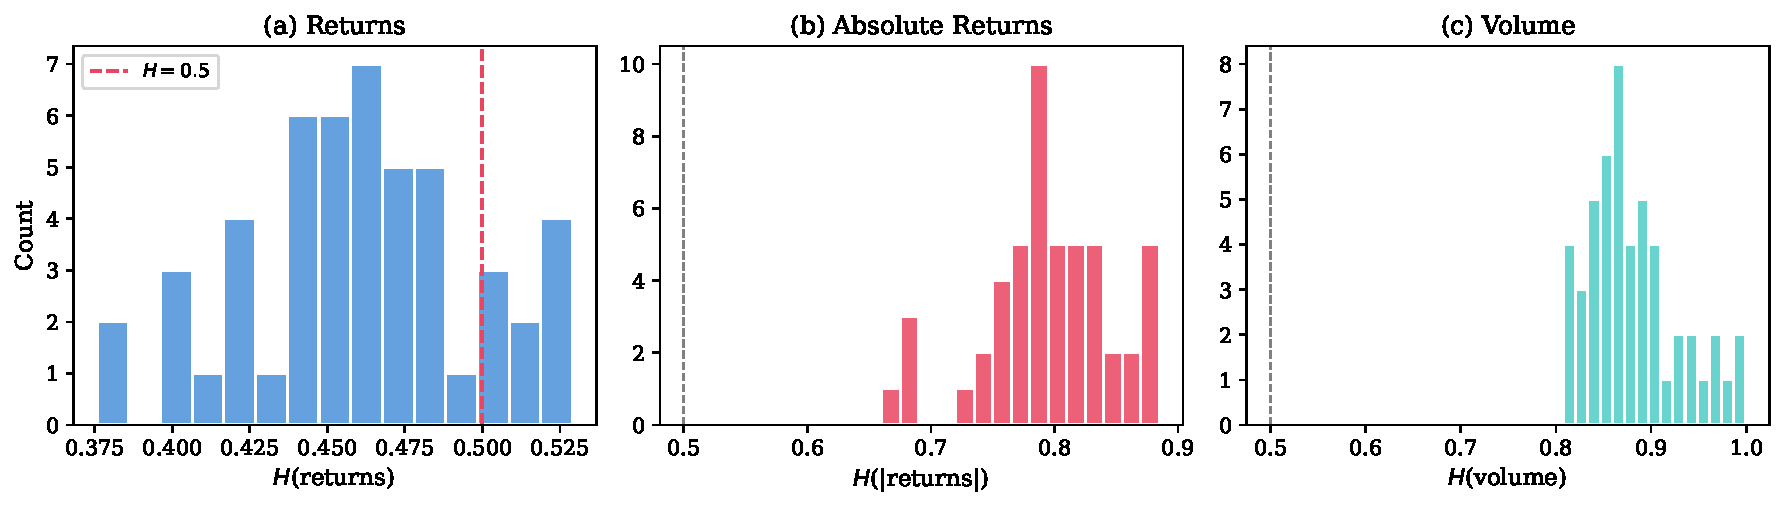
\includegraphics[width=\textwidth]{figures/fig1_hurst_distributions.pdf}
\caption{Distribution of full-sample Hurst exponents across 50 S\&P~500 constituents (2015--2026). (a)~Returns cluster around $H = 0.5$. (b)~Absolute returns show strong long memory ($H \approx 0.8$). (c)~Volume exhibits the strongest persistence ($H \approx 0.9$).}
\label{fig:distributions}
\end{figure}

\begin{figure}[H]
\centering
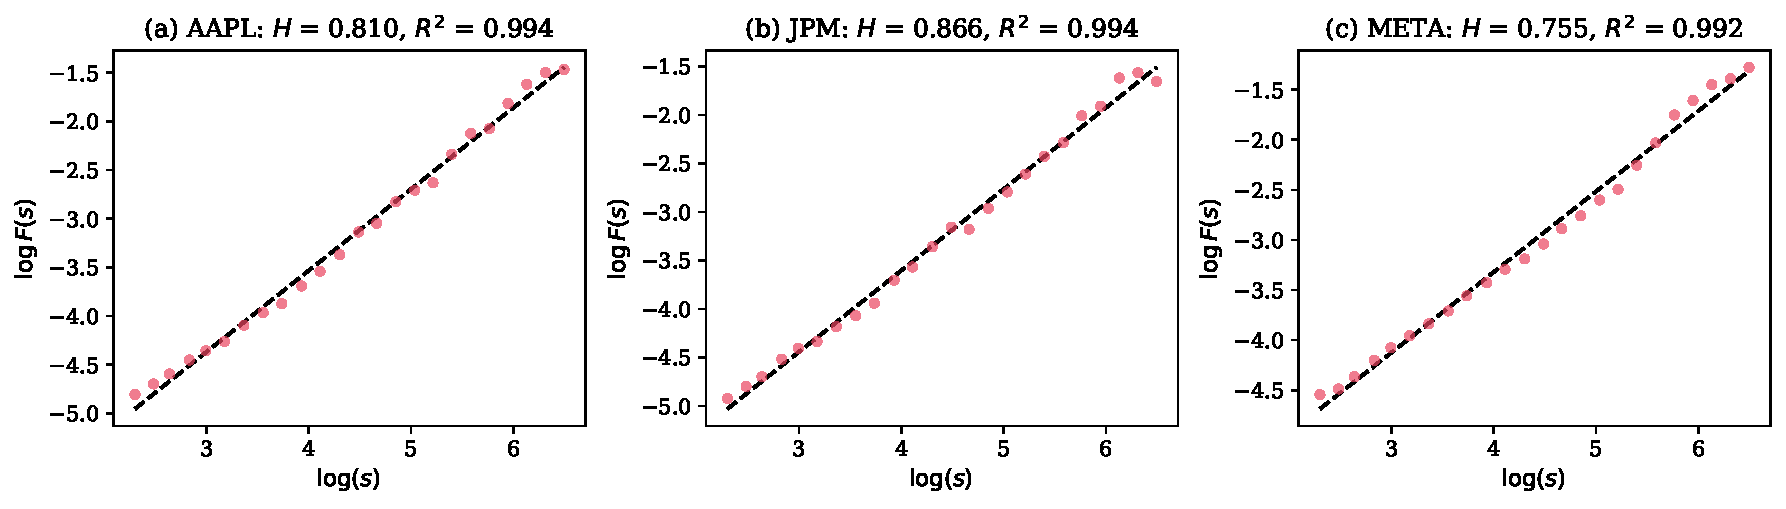
\includegraphics[width=\textwidth]{figures/fig2_loglog_dfa.pdf}
\caption{Log-log DFA plots for absolute returns (AAPL, JPM, META). High $R^2$ values confirm excellent linearity.}
\label{fig:loglog}
\end{figure}

\begin{figure}[H]
\centering
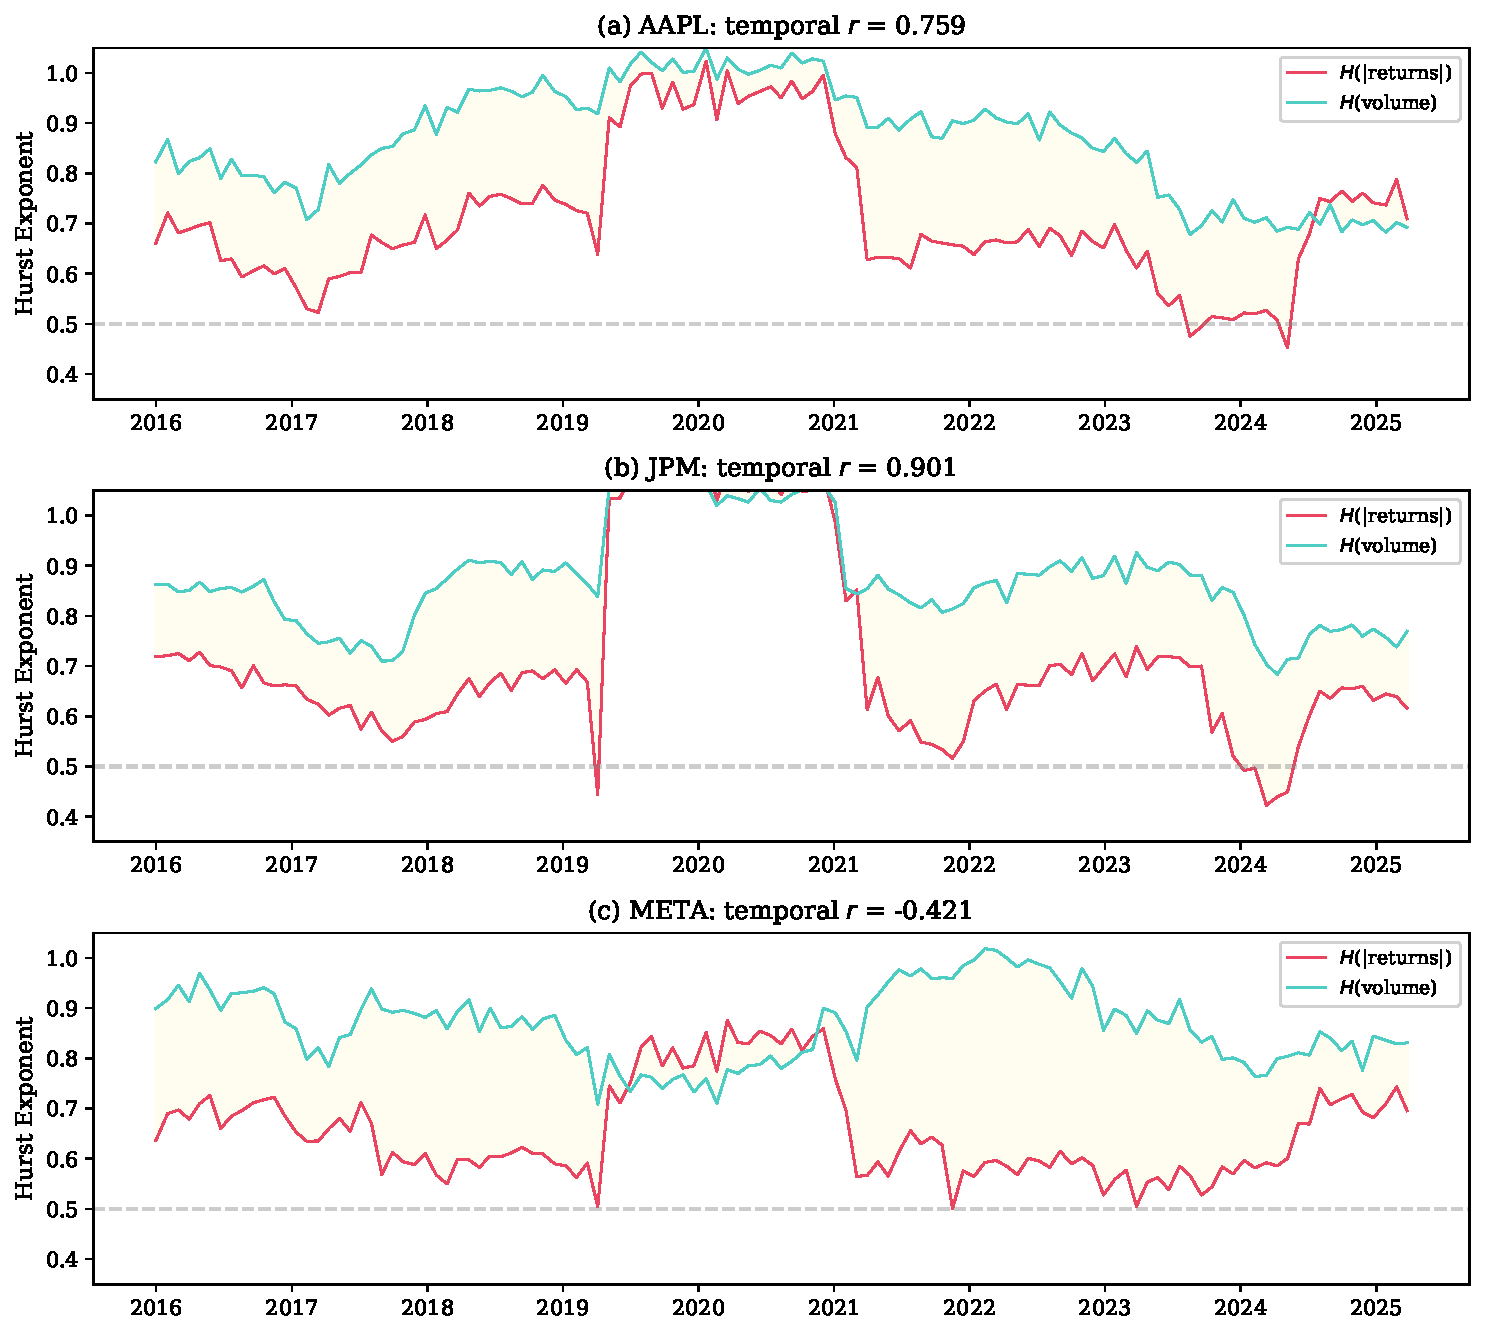
\includegraphics[width=0.85\textwidth]{figures/fig3_rolling_hurst_exemplars.pdf}
\caption{Rolling Hurst exponents for $H^{(i)}_{|r|,t}$ (red) and $H^{(i)}_{v,t}$ (teal). (a)~AAPL: $r = 0.759$. (b)~JPM: $r = 0.901$. (c)~META: $r = -0.421$ (negative coupling during corporate restructuring).}
\label{fig:rolling}
\end{figure}

\begin{figure}[H]
\centering
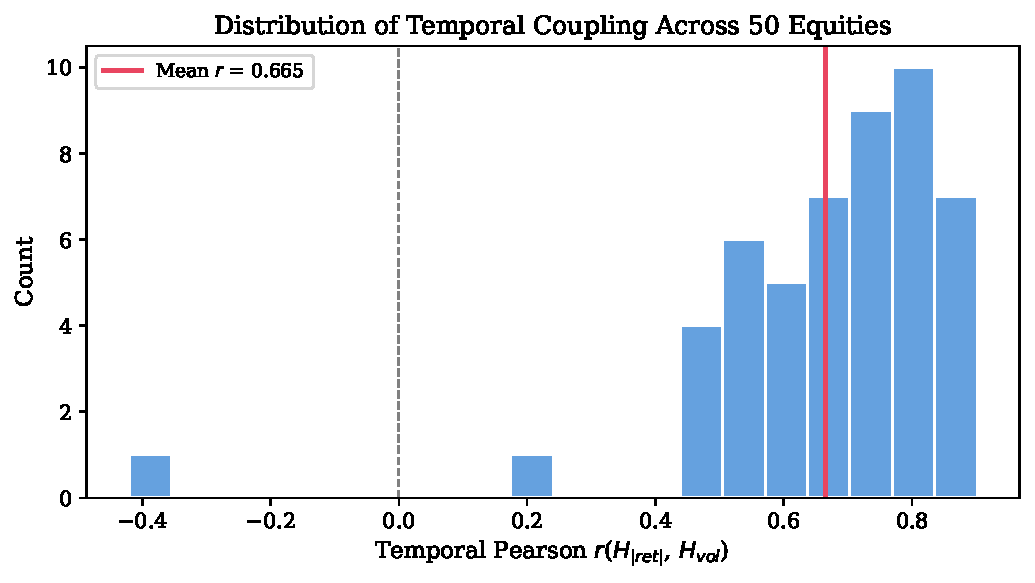
\includegraphics[width=0.75\textwidth]{figures/fig4_temporal_correlation_distribution.pdf}
\caption{Distribution of temporal coupling across 50 equities. Mean $r = 0.665$; META is the sole outlier.}
\label{fig:temporal_dist}
\end{figure}

\begin{figure}[H]
\centering
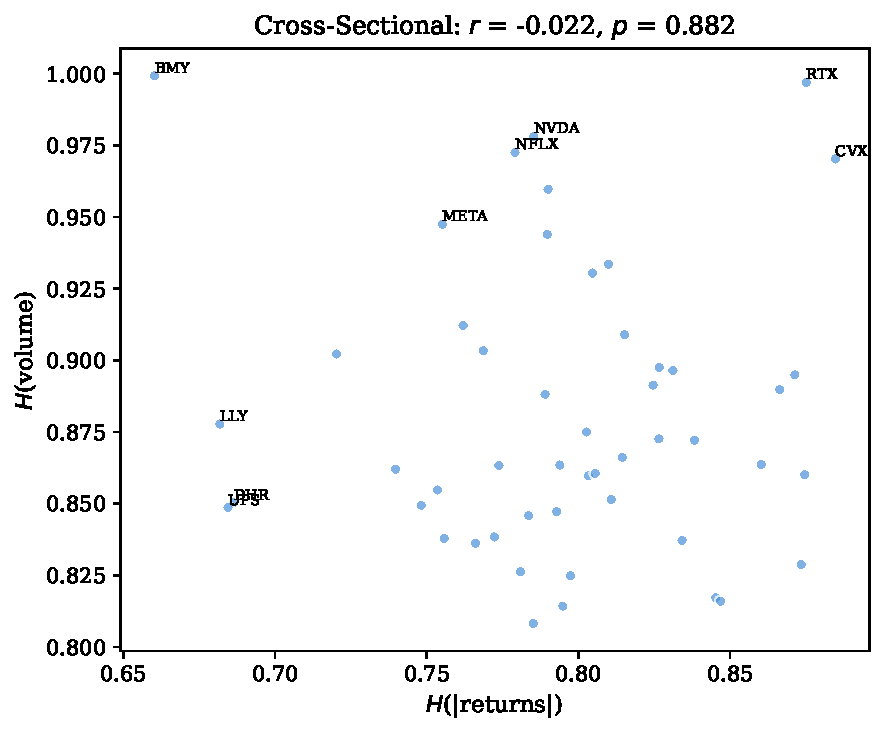
\includegraphics[width=0.65\textwidth]{figures/fig5_cross_sectional_scatter.pdf}
\caption{Cross-sectional scatter: $H^{(i)}_{|r|}$ vs.\ $H^{(i)}_{v}$. No relationship ($r = -0.02$, $p = 0.88$).}
\label{fig:cross_sectional}
\end{figure}

\begin{figure}[H]
\centering
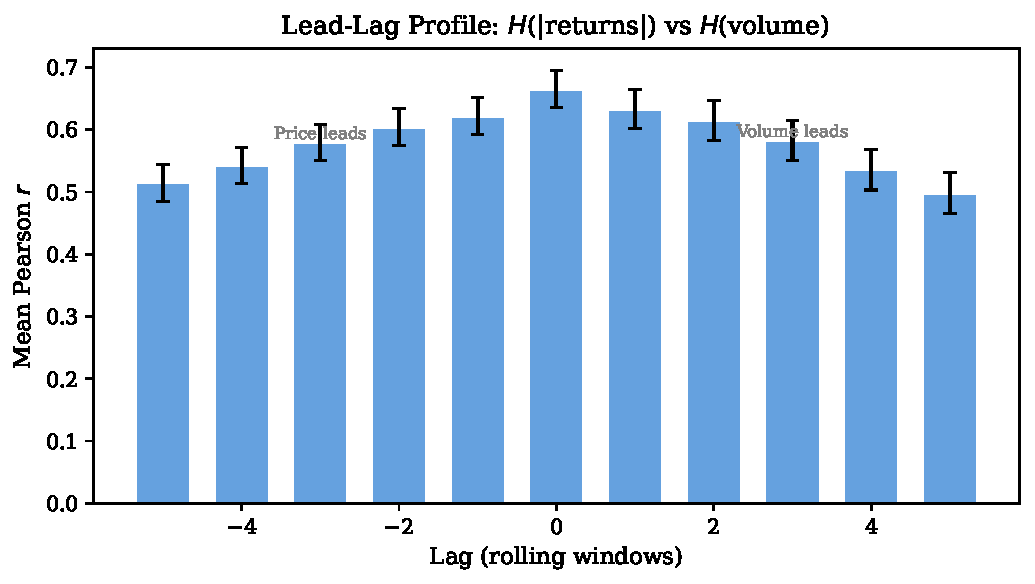
\includegraphics[width=0.75\textwidth]{figures/fig6_lead_lag_profile.pdf}
\caption{Average lead-lag cross-correlation profile across 50 equities. Lag zero is dominant; decay is symmetric.}
\label{fig:leadlag}
\end{figure}

\begin{figure}[H]
\centering
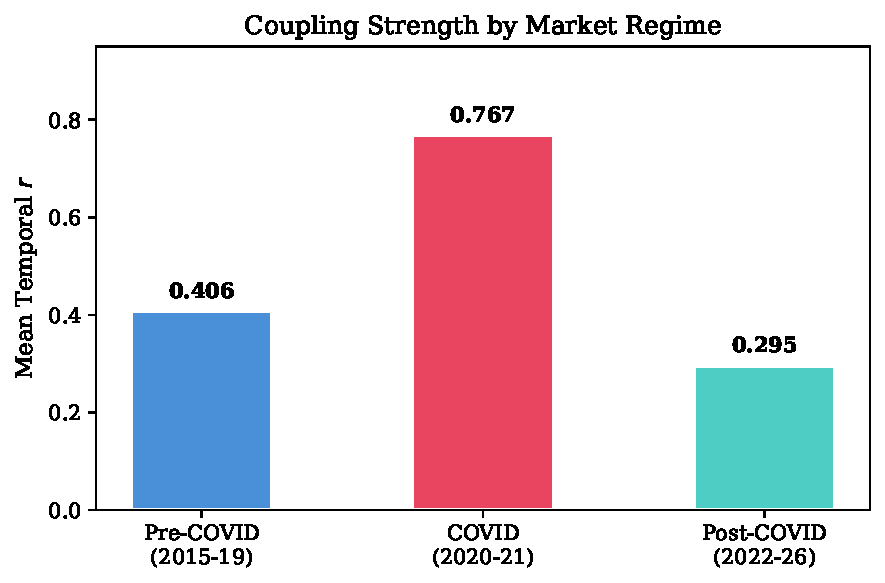
\includegraphics[width=0.65\textwidth]{figures/fig7_subperiod_analysis.pdf}
\caption{Temporal coupling by market subperiod. Coupling nearly doubles during COVID ($r = 0.77$) relative to the pre-COVID baseline ($r = 0.41$).}
\label{fig:subperiod}
\end{figure}

\begin{figure}[H]
\centering
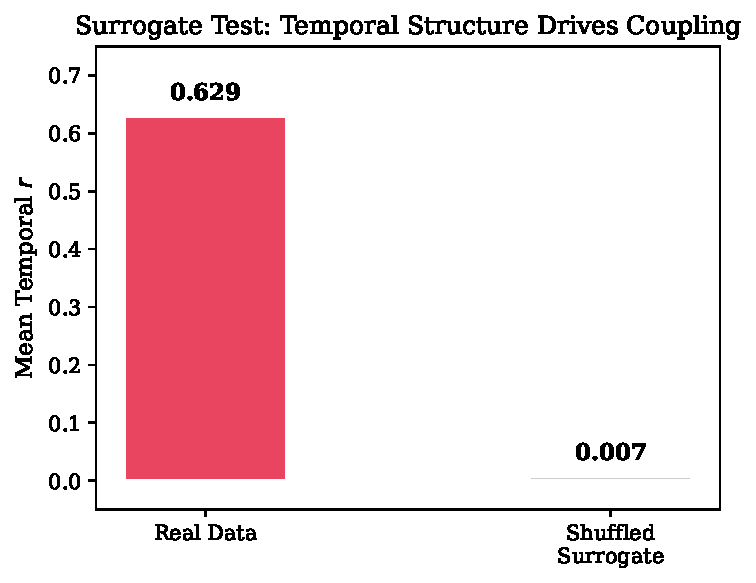
\includegraphics[width=0.55\textwidth]{figures/fig8_surrogate_test.pdf}
\caption{Surrogate test. Shuffling each series independently destroys coupling ($r = 0.629 \to 0.007$), confirming the temporal origin of the co-movement.}
\label{fig:surrogate}
\end{figure}

\begin{figure}[H]
\centering
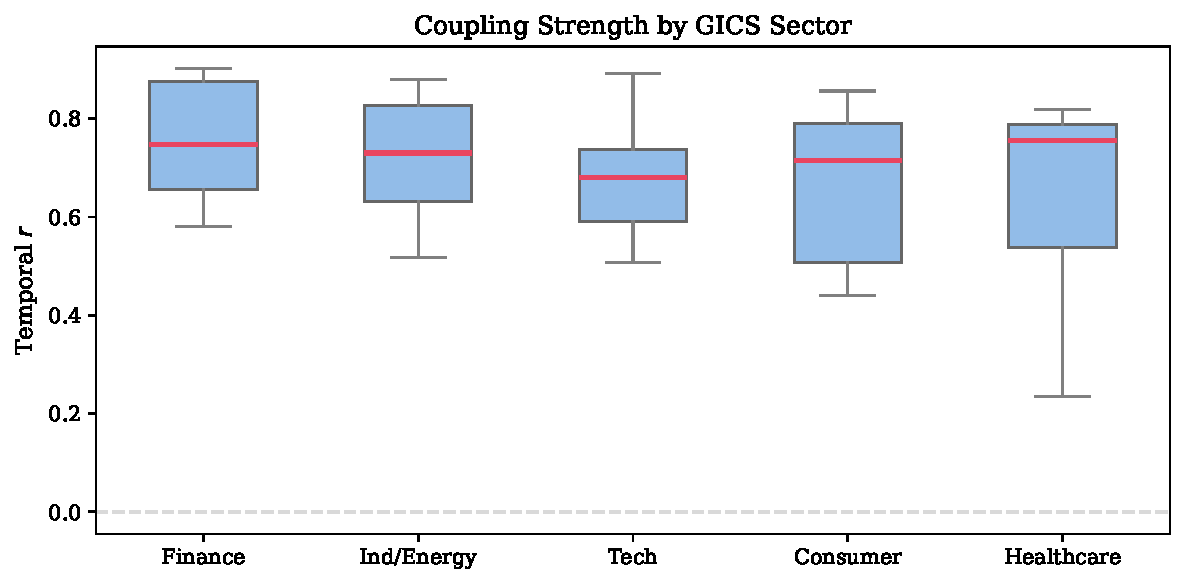
\includegraphics[width=0.85\textwidth]{figures/fig9_sector_decomposition.pdf}
\caption{Temporal coupling by GICS sector. Present across all sectors; Finance is strongest ($r = 0.756$).}
\label{fig:sectors}
\end{figure}

% ============================================================
\appendix
% ============================================================

\section{Sample Composition}
\label{app:tickers}

\begin{table}[H]
\centering
\small
\caption{The 50 S\&P~500 constituents used in this study, with GICS sector classification.}
\label{tab:tickers}
\begin{tabular}{lll}
\toprule
Ticker & Company & Sector \\
\midrule
AAPL & Apple & Technology \\
MSFT & Microsoft & Technology \\
AMZN & Amazon & Consumer Discretionary \\
GOOGL & Alphabet & Technology \\
META & Meta Platforms & Technology \\
TSLA & Tesla & Consumer Discretionary \\
NVDA & NVIDIA & Technology \\
JPM & JPMorgan Chase & Financials \\
V & Visa & Financials \\
JNJ & Johnson \& Johnson & Healthcare \\
WMT & Walmart & Consumer Staples \\
PG & Procter \& Gamble & Consumer Staples \\
MA & Mastercard & Financials \\
UNH & UnitedHealth & Healthcare \\
HD & Home Depot & Consumer Discretionary \\
DIS & Walt Disney & Communication Services \\
BAC & Bank of America & Financials \\
XOM & ExxonMobil & Energy \\
CSCO & Cisco Systems & Technology \\
VZ & Verizon & Communication Services \\
INTC & Intel & Technology \\
CMCSA & Comcast & Communication Services \\
PFE & Pfizer & Healthcare \\
ABT & Abbott Laboratories & Healthcare \\
CRM & Salesforce & Technology \\
NKE & Nike & Consumer Discretionary \\
MRK & Merck & Healthcare \\
T & AT\&T & Communication Services \\
PEP & PepsiCo & Consumer Staples \\
TMO & Thermo Fisher & Healthcare \\
COST & Costco & Consumer Staples \\
AVGO & Broadcom & Technology \\
CVX & Chevron & Energy \\
ABBV & AbbVie & Healthcare \\
ACN & Accenture & Technology \\
MCD & McDonald's & Consumer Discretionary \\
LIN & Linde & Materials \\
TXN & Texas Instruments & Technology \\
QCOM & Qualcomm & Technology \\
LOW & Lowe's & Consumer Discretionary \\
NEE & NextEra Energy & Utilities \\
HON & Honeywell & Industrials \\
UPS & United Parcel Service & Industrials \\
MS & Morgan Stanley & Financials \\
BMY & Bristol-Myers Squibb & Healthcare \\
RTX & RTX (Raytheon) & Industrials \\
AMGN & Amgen & Healthcare \\
CAT & Caterpillar & Industrials \\
GS & Goldman Sachs & Financials \\
BLK & BlackRock & Financials \\
\bottomrule
\end{tabular}
\end{table}

\section{Replication Guide}
\label{app:replication}

All code, data scripts, and the manuscript source are archived at Zenodo (concept DOI: \href{https://doi.org/10.5281/zenodo.19611543}{10.5281/zenodo.19611543}, always resolving to the latest version; this submission corresponds to v1.1.0, version DOI \href{https://doi.org/10.5281/zenodo.19835451}{10.5281/zenodo.19835451}) and on GitHub at \url{https://github.com/mhdk1602/fractal-pv-coupling}. The repository contains a Python package (\texttt{fractal\_pv}) installable via \texttt{pip install -e .} with Python~3.10 or later. Dependencies are pinned in \texttt{pyproject.toml}.

The replication workflow proceeds as follows. (1)~\texttt{fractal\_pv.data.fetch\_universe()} downloads daily OHLCV data for all 50 tickers from Yahoo Finance and caches them as parquet files under \texttt{data/raw/}. (2)~\texttt{fractal\_pv.stationarity.prepare\_series()} transforms raw prices into log-returns, absolute log-returns, and log-volume, with ADF/KPSS stationarity verification. (3)~\texttt{fractal\_pv.hurst.estimate\_dfa()} computes full-sample Hurst exponents; \texttt{bootstrap.block\_bootstrap\_hurst()} produces confidence intervals. (4)~\texttt{fractal\_pv.rolling.rolling\_dual\_hurst()} computes aligned rolling $H^{(i)}_{|r|,t}$ and $H^{(i)}_{v,t}$ series. (5)~\texttt{fractal\_pv.predict.compute\_coupling\_intensity()} derives CII; \texttt{compute\_forward\_metrics()} computes outcome variables. (6)~\texttt{fractal\_pv.predict.build\_prediction\_panel()} assembles the panel; \texttt{inference\_robust.robust\_panel\_regression()} estimates coefficients with all five standard-error specifications. (7)~\texttt{fractal\_pv.regimes} conditions on VIX and crisis windows. Figures are generated via matplotlib and saved to \texttt{research/paper/figures/}. The manuscript compiles with \texttt{tectonic main.tex} or any standard \LaTeX\ distribution.

\bibliographystyle{elsarticle-harv}
\bibliography{references}

\end{document}
